%%%%%%%%%%%%%%%%%%%%%%%%%%%%%%%%%%%%%%%%%%%%%%
\section{PDS electronics}\label{sec:pds-elec-daq}

\fixme{this section needs some language editing}

Scintillation light from LAr comes from the two different excited 
states with lifetimes of about 6 ns and 1.6 $\mu$s. 
Only a limited amount of light is collected by this system, so we 
assume the electronics must be designed to collect the light 
from both excited states. A summary of the general requirements 
for the system, including initial requirements from a 
physics performance perspective, are given in Table~\ref{tab:fee_req}.
%
\begin{table*}[ht]
\centering
%\vspace{4mm}
\begin{tabular}{| l | l |} \hline
 Performance Parameter       & Target   \cr   \hline
 Time Resolution                   & Better than 30 ns wrt event time zero ("t0")      \cr  \hline
 Charge Resolution               & 0.25\% photo-electron equivalent                     \cr \hline
 Dynamic Range                   & $\sim$ x10 better than detector (1000:1)          \cr \hline
 Linearity                               & Sufficient to resolve 1 photo-electron signals   \cr    \hline
 Multi-Hit Capability              & Sufficient to measure Triplet (late) Photons          \cr   \hline
 Dead Time                           & Live up to 2 drift times either side of beam spill          \cr    \hline
 Bias Control                        & 0.1 V resolution up to 30 V per channel  \cr    \hline
 Calibration                          & On-board Charge Injection  \cr    \hline
 Timing                                 & Events time-stamped using NO$\nu$A Timing or equivalent syst.  \cr    \hline
\end{tabular}
\caption{\label{tab:fee_req} Physics Requirements for the Photon Detector Electronics.}
\end{table*}
%
The plans for the electronics for the photon detection subsystem 
include a baseline design with several options 
that remain R\&D activities.   

In the baseline plan, there are no front-end electronics in the cold volume.  
The un-amplified signals from the SiPMs 
are transmitted to outside the cryostat %on cables 
for processing and digitization, with
the advantage that the infrastructure required for inside the cryostat is 
reduced (power, data cables, precision clocks, data protocols, etc.).  
%
A custom module, called the SiPM Signal Processor (SSP), receives the SiPM signals. % has been designed and built 
%for preprocessing for trigger and data acquisition (DAQ) in the front-end.
%to perform signal processing in the front-end as preprocessing for trigger and data acquisition (DAQ). 
%The module is called the SiPM Signal Processor (SSP).  

An SSP consists of 12 readout channels packaged in a self-contained 
1U module.  
Each channel contains a fully-differential voltage amplifier and a 
14-bit, 150 MSPS analog-to-digital converter (ADC) that 
digitizes the waveforms received from the SiPMs.  
The front-end amplifier is configured as fully-differential with high common-mode 
rejection, and receives the SiPM signals into a termination resistor that 
matches the characteristic impedance of the signal cable. 
Currently there is no shaping of the signal, since the SiPM response 
is slow enough relative to the speed of the digitization to obtain 
several digitized samples of the leading edge of the pulse for the determination of signal timing.  

The digitized data is stored in pipelines in the SSP, for up to $\sim$ 13 $\mu$s.  
The processing is pipelined, and performed by a Xilinx Artix-7 
Field-Programmable Gate Array (FPGA).  
The FPGA implements an independent Data Processor (DP) for each channel.  
The processing incorporates a leading edge discriminator for detecting events
and a constant fraction discriminator (CFD) for sub 
clock timing resolution.  
Because the FPGA is programmable and accessible, it is possible to explore 
different data processing algorithms and techniques, and even customize the 
readout for a given type of event (supernova for example.)  
A picture of the module is shown in Fig.~\ref{fig:PD_fig-e-2}.  
A block diagram of the system is shown in Fig.~\ref{fig:PD_fig-e-3}.
%Fig. xx3.  Picture of the SSP module.
%
\begin{cdrfigure}[SSP Photograph]{PD_fig-e-2}{Picture of SSP module.}
  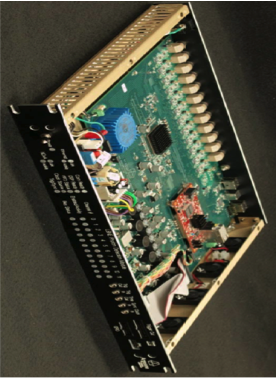
\includegraphics[angle=90,width=0.5\textwidth]{PD_fig-e-2.png}
\end{cdrfigure}

\begin{cdrfigure}[SSP Block Diagram]{PD_fig-e-3}{Block diagram of the SSP Module.}
  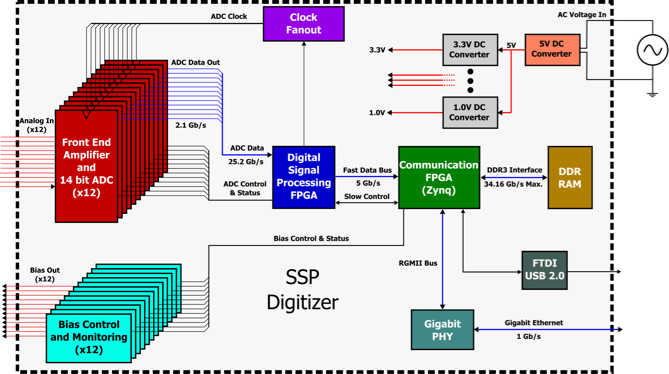
\includegraphics[width=0.8\textwidth]{PD_fig-e-3.png}
\end{cdrfigure}
%
In the simplest mode of operation, the module can perform waveform capture, 
using either an internal trigger or an external trigger.  
Up to 2046 waveform samples may be read out for each event.  When waveform 
readouts overlap the device can be configured to offset, 
truncate or completely suppress the overlapping waveform.  
Pile-up events can also be suppressed.  

Generally, the SSP performs pipelined processing.  
The module has been designed to support several different triggering schemes, 
including self-triggered, use of an external trigger, or use an 
external gate to readout all events within a time-window.  
In order for the events measured in the photon detector to be matched up 
with the corresponding events in the TPC, the front-end electronics 
attaches a timestamp to the data as it is acquired.  
The timestamp is unique, and has a correspondence with the timestamps in 
the TPC electronics processing.  
The timestamp in the SSP is applied to the event data as it is digitized, 
and becomes part of the data as the processing proceeds.  
In the case where zero-suppression and data sparsification are used, 
the timestamp on accepted data remains intact.  
To achieve this, the TPC and PD electronics must be synchronized, 
including timestamp counter resets, and a known and stable calibration between 
the corresponding timing resolution of the ADC conversion in the two systems.  

A Xilinx Zynq FPGA, onboard the MicroZed system-on-module, handles the 
slow control and event data transfer.  
The SSP has two parallel communication interfaces; USB 2.0 and 10/100/1000 Ethernet.  
The 1 Gb/s Ethernet supports full TCP/IP protocol.  
The module includes a separate 12-bit high-voltage DAC for each channel to 
provide up to 30 V of bias to each SiPM.  
The module also feature charge injection for performing diagnostics and linearity 
monitoring, and also voltage monitoring.

In tests to date, the SSP is capable of measuring single photo-electron signals 
coming from the SiPMs over a cable length of 30 meters when the SiPMs are 
operated at LAr temperatures.  
The timing resolution of the signals has been measured to be better than 3 ns.  
The full-differential signal processing in the front-end circuitry 
is important in achieving this result.

The baseline plan assumes that three SiPM signals can be ganged 
together into one readout channel. 
By using a multi-conductor cable with four twisted pairs, this 
results in one cable per PD consisting of 12 SiPMs.      

